%!TEX root = ..\..\main.tex

\section{Diskussion}
\label{sec:Auswertung}
\todo[inline, color=yellow]{Artjom}

Nach der radialen Entzerrung mit dem implementierten Verfahren kommt man zu dem in Abb. \ref{fig:Ergebnis} und Abb. \ref{fig:diffsResult} gezeigten Ergebnis. Die Koeffizienten der radialen Entzerrung sind für dieses Resultat in Gl. \ref{equ:radial_koeff} notiert. 

\begin{align}
a &=  2.8974105705613364E-8 \nonumber \\
b &= -4.0458117860182954E-15 \nonumber \\
c &=  2.8527492714683317E-21
\label{equ:radial_koeff}
\end{align}

\begin{figure}[H]
	\subfigure{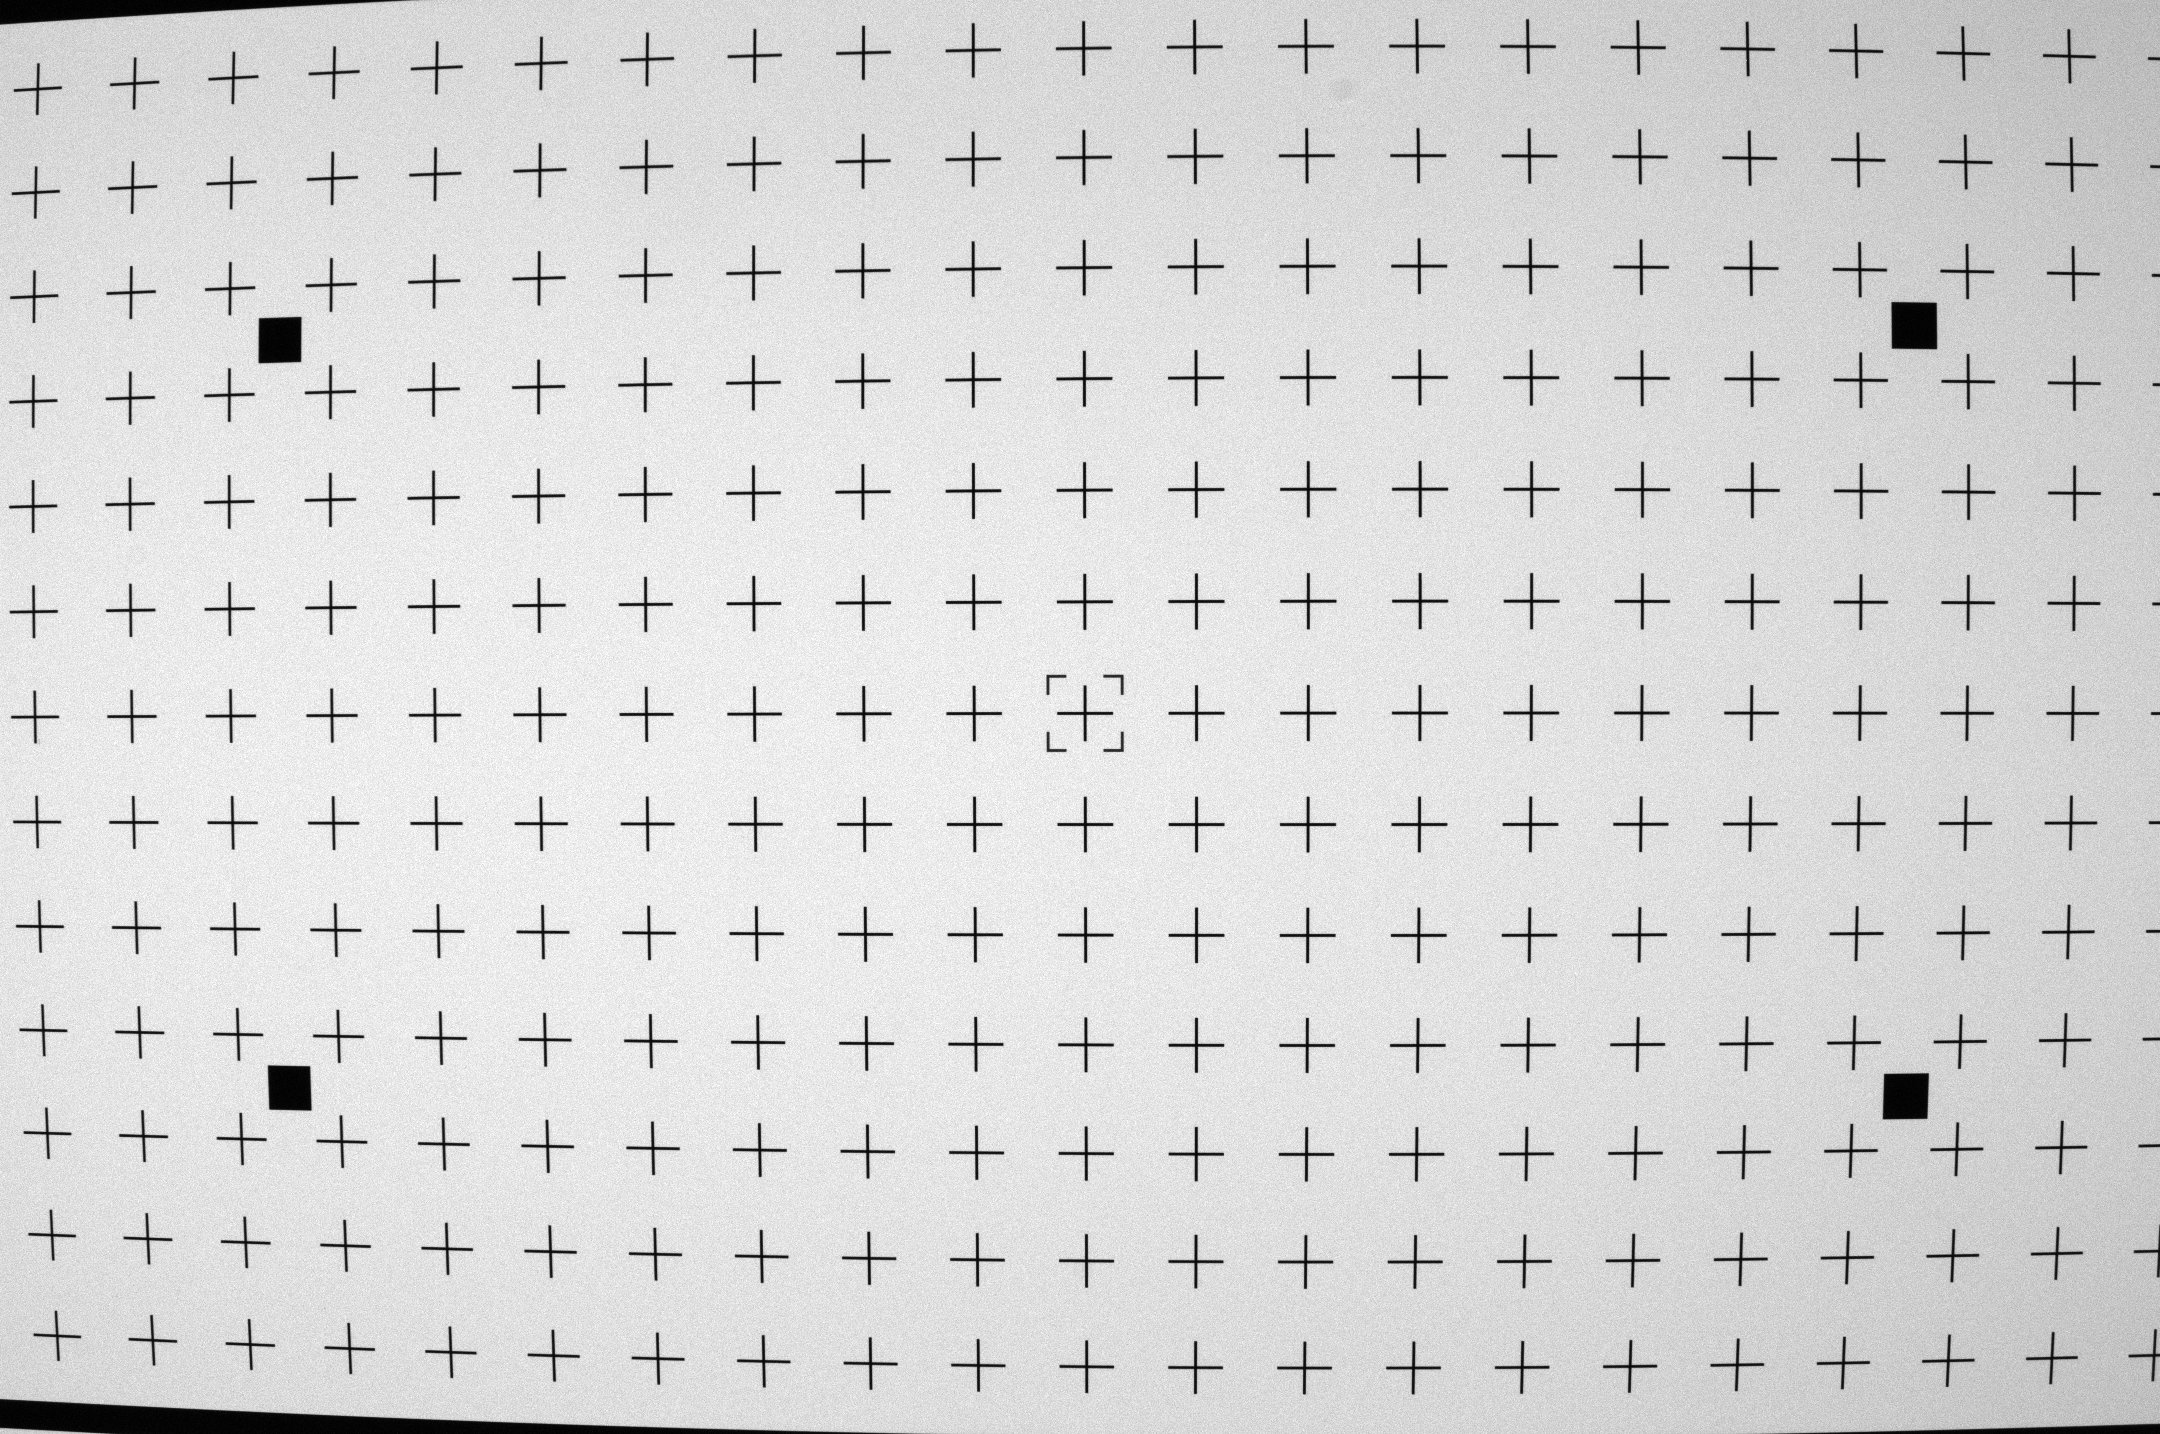
\includegraphics[width=\textwidth/2]{Images/Auswertung/Testbild1/18mm_11-1.jpg}}
	\subfigure {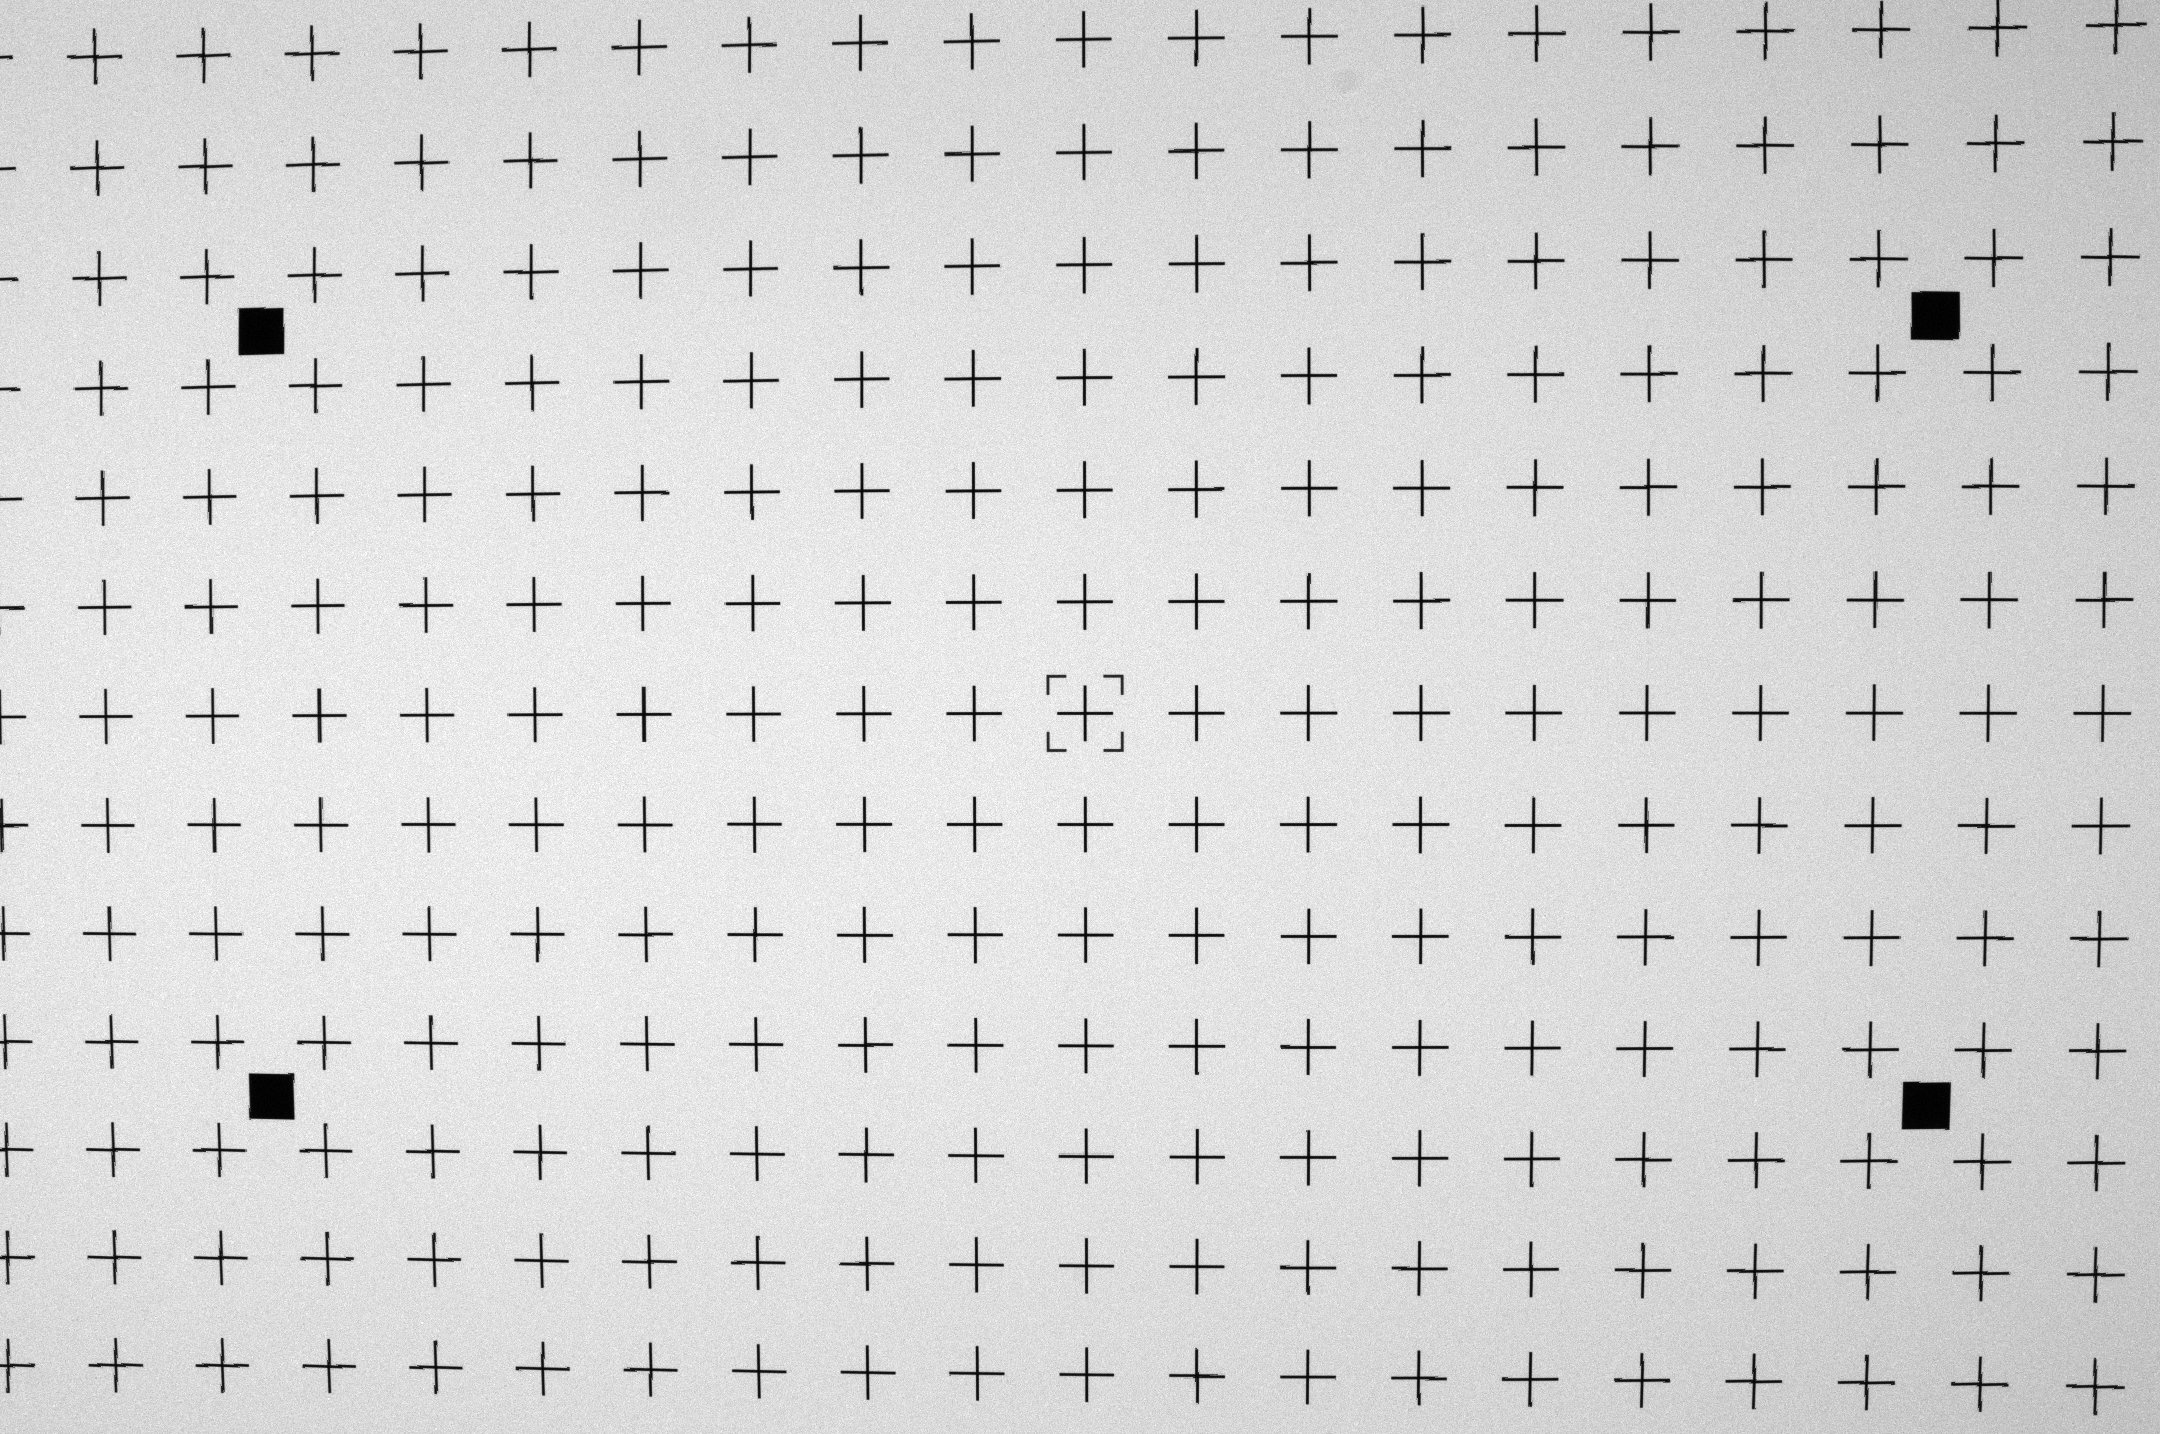
\includegraphics[width=\textwidth/2]{Images/Auswertung/Testbild1/Radial.jpg}}
	\caption{Links: Ausgangsbild. Rechts: Resultat der Radialen Entzerrung}
	\label{fig:Ergebnis}
\end{figure}
	
Anhand der Abb. \ref{fig:Ergebnis} ist deutlich zu erkennen, dass das Gitter gleichmäßiger und gerader wird. Des Weiteren wird durch Abb. \ref{fig:diffsResult} verdeutlicht, dass sich die Differenzen zwischen Start- und Zielkoordinaten der Punkte verkleinern. Dies bestätigt, dass das Verfahren funktioniert.

\begin{figure}[H]
	\subfigure {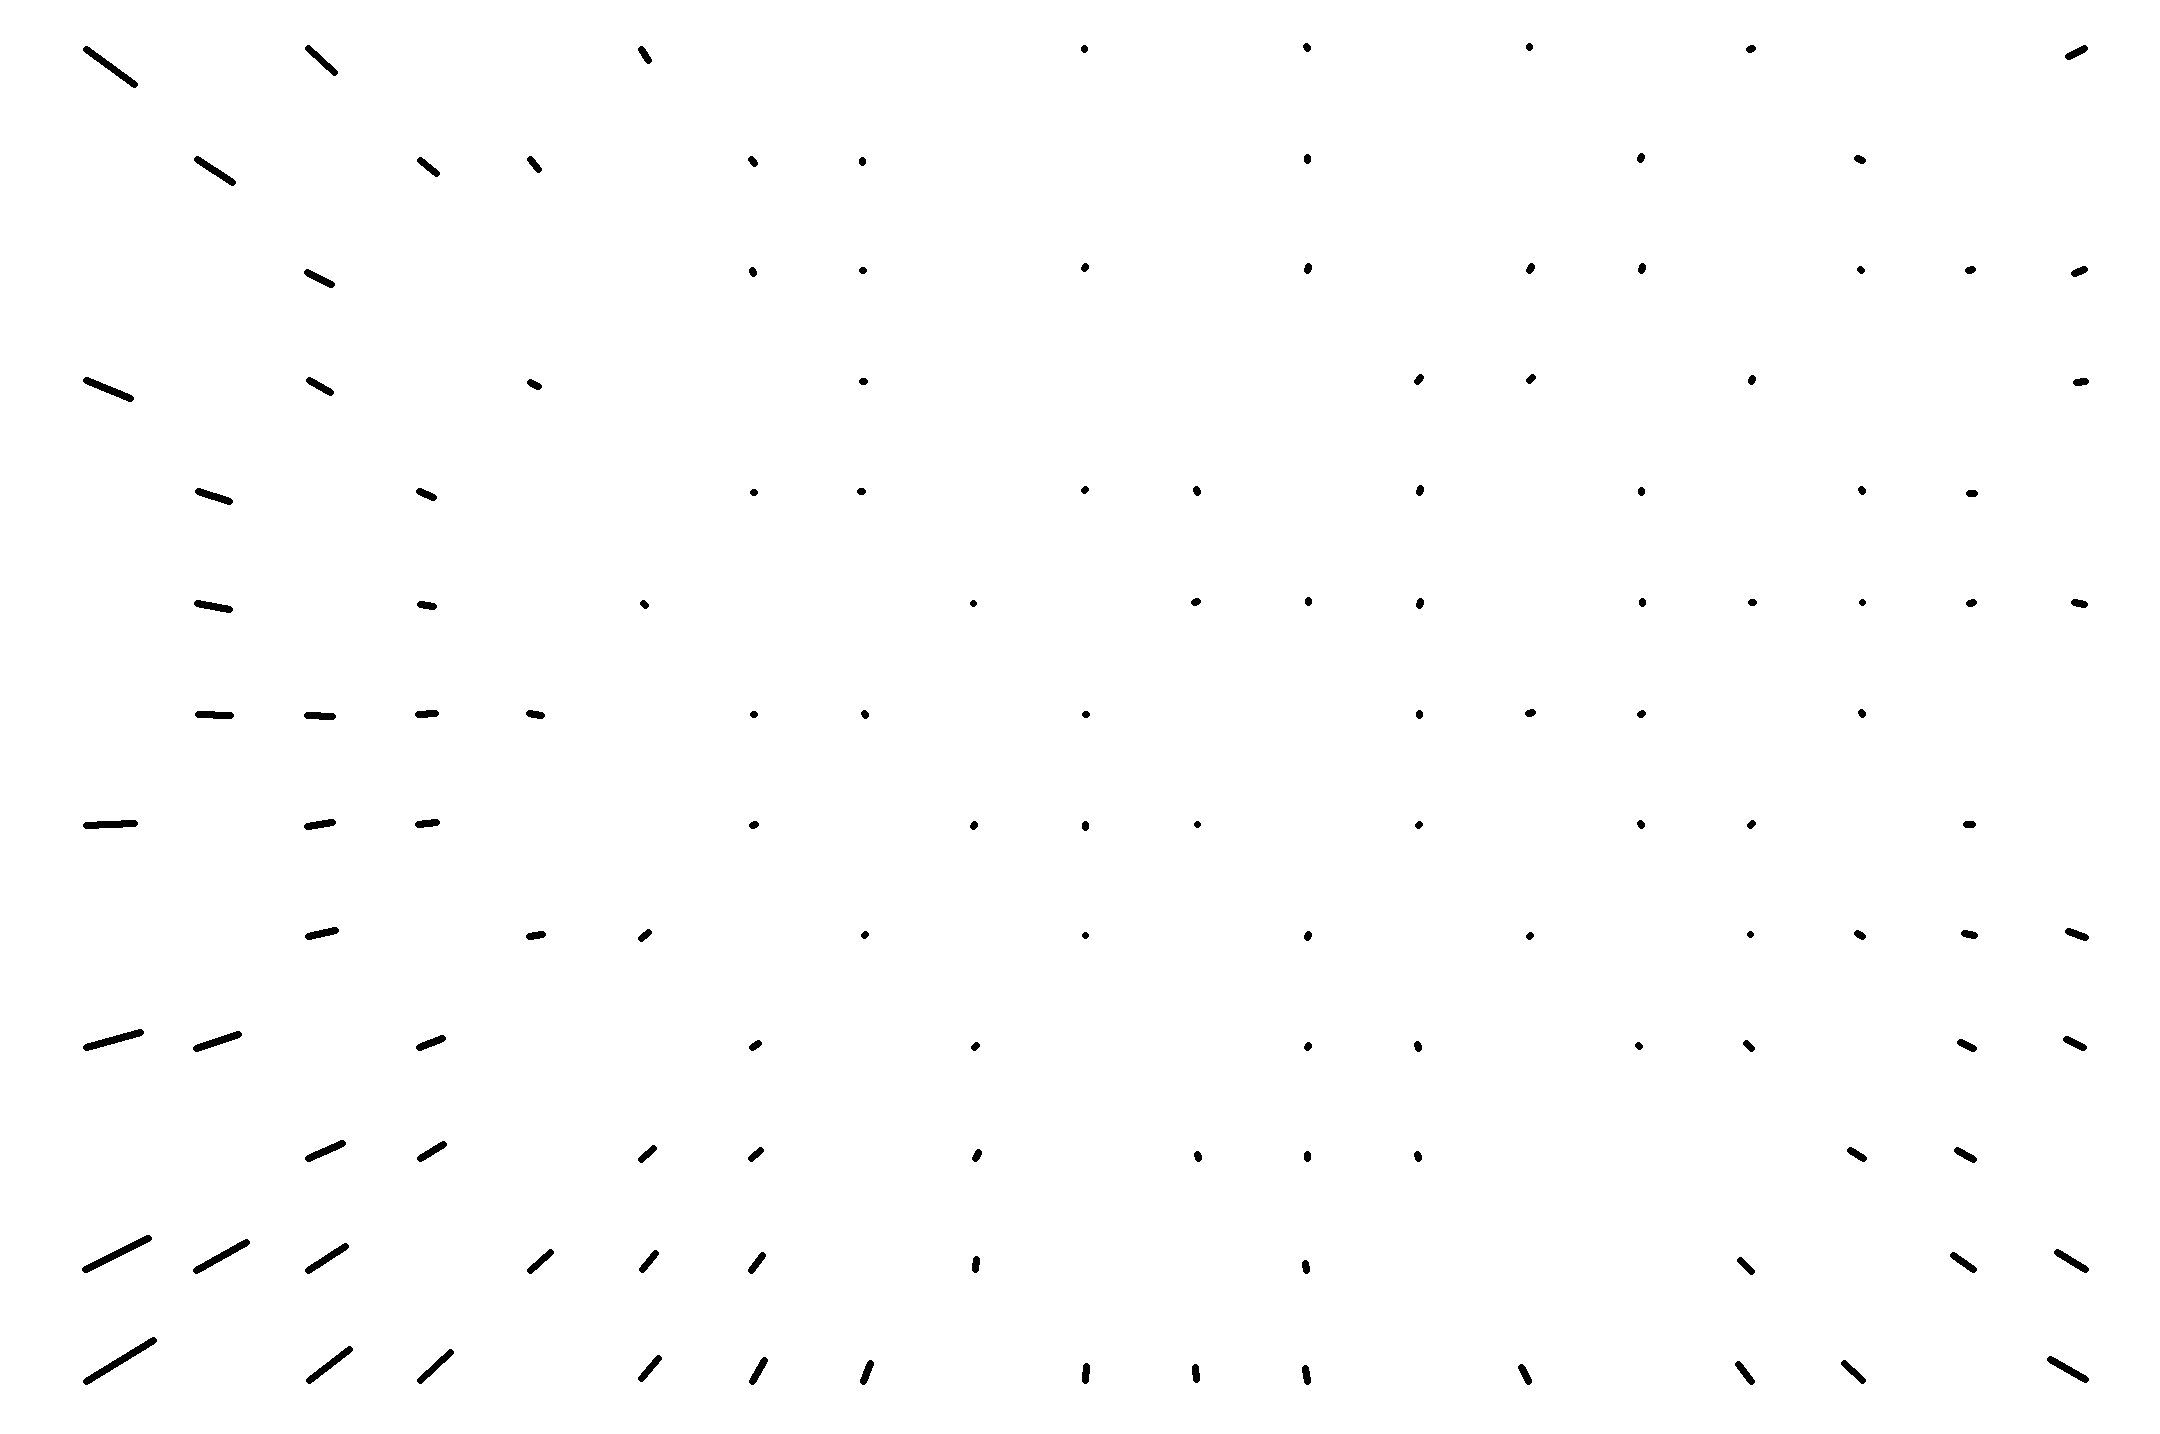
\includegraphics[width=\textwidth/2]{Images/Auswertung/Testbild1/SourceImage with PointPairs_onlydiffs.jpg}}
	\subfigure{	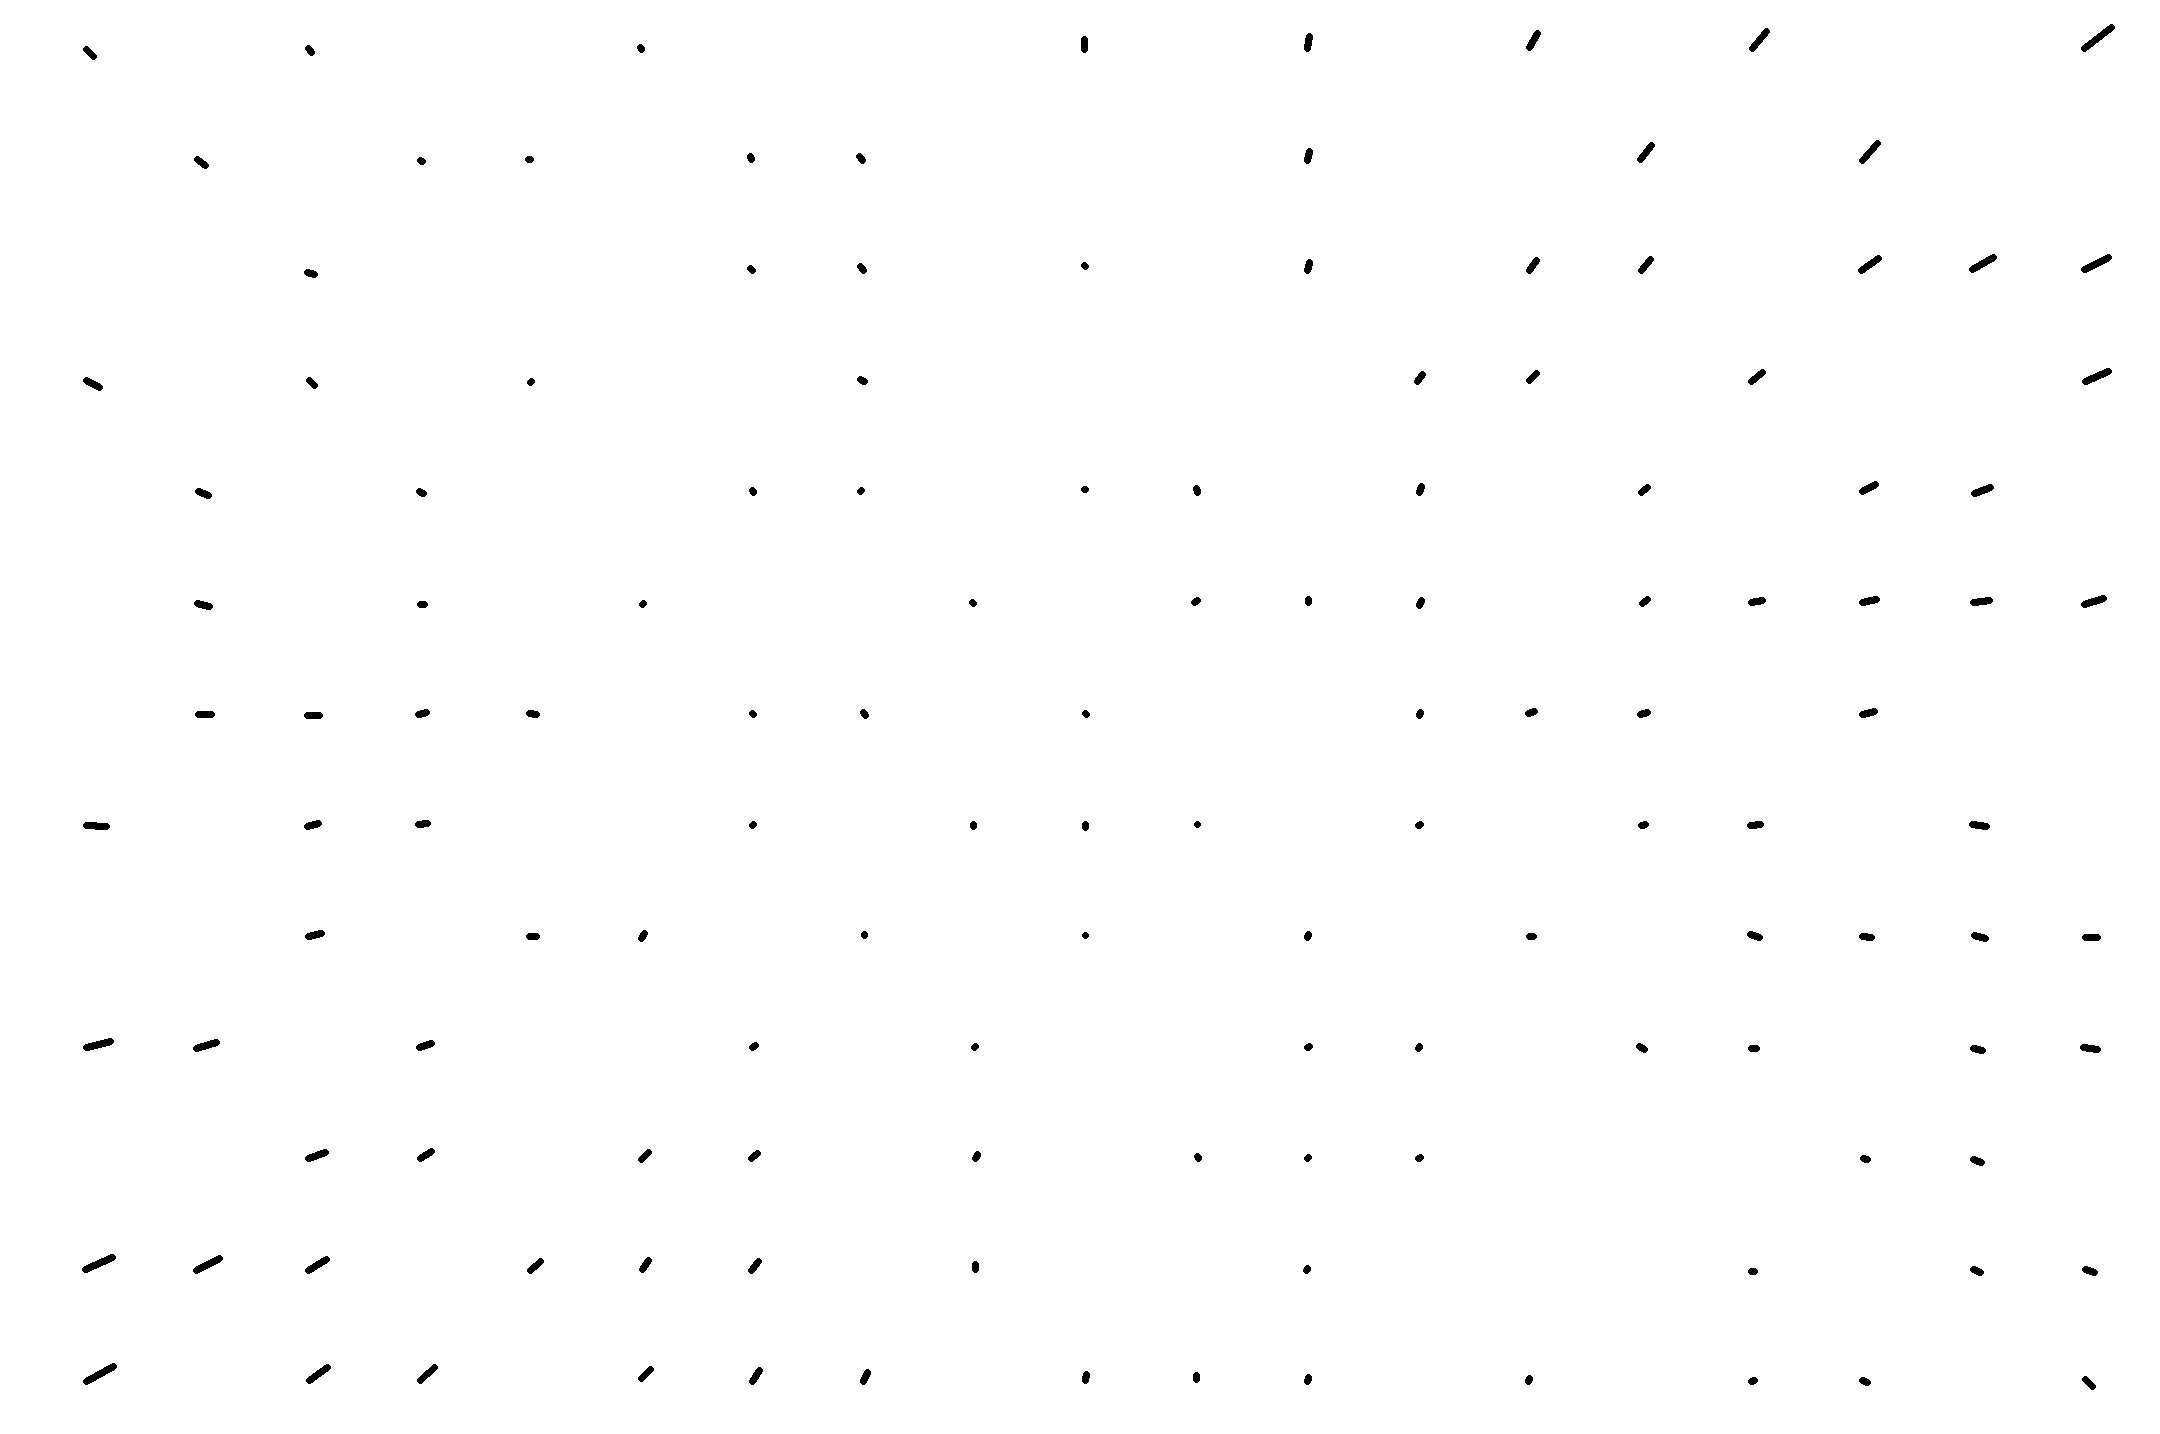
\includegraphics[width=\textwidth/2]{Images/Auswertung/Testbild1/Radial_onlydiffs.jpg}}
	\caption{Links: Differenzen zwischen den idealen und realen Stützpunkten. \\Rechts: Differenzen zwischen den idealen und transformierten Stützpunkten.}
	\label{fig:diffsResult}
\end{figure}

Bei genaurer Betrachtung der Differenzen in Abb. \ref{fig:diffsResult} ist jedoch zu erkennen, dass sich vor allem im linken Bereich die Differenzen verkleinern, wohingegen sie im rechten Bereich etwas zunehmen.
Dies deutet darauf hin, dass das Ergebnis noch nicht optimal ist. Einer der Gründe ist
das implementierte Verfahren zur radialen Entzerrung. Es funktioniert nur wenn in dem Bild nur eine vom Radius abhängige Verzerrung existiert. Wie man jedoch in Abb. \ref{fig:diffsResult} erkennen kann ist die Verzerrung auf der linken Seite größer als auf der rechten Seite.
Es existiert somit eine zusätzliche perspektivische Verzerrung für die eine vorherige projektive Transformation notwendig ist damit das implementierte Verfahren angewendet werden kann.

%@VERA Stimmt das so?
Weiterhin ist für das Verfahren problematisch, wenn die Verzerrung im mittleren Radius größer ist als im äußeren Radius (Fish-Eye-Effekt), da dass Verfahren mit einer zum Radius zunehmenden Verzerrung rechnet. Bei diesem Effekt sind aber die äußeren Start und Ziel-Koordinaten bereits sehr nah bei einander, welches vom Optimierer nicht bereits weiter verbessert werden kann.

Ein zusätzlicher Nachteil der Implementierung ist das setzen der Punktpaare. Dies ist nicht sehr praxisnah, da im Optimalfall das Gitter berechnet werden kann. Zusätzlich bringt es Ungenauigkeiten in der Berechnung der Entzerrung.

